% Options for packages loaded elsewhere
\PassOptionsToPackage{unicode}{hyperref}
\PassOptionsToPackage{hyphens}{url}
%
\documentclass[
]{book}
\usepackage{lmodern}
\usepackage{amssymb,amsmath}
\usepackage{ifxetex,ifluatex}
\ifnum 0\ifxetex 1\fi\ifluatex 1\fi=0 % if pdftex
  \usepackage[T1]{fontenc}
  \usepackage[utf8]{inputenc}
  \usepackage{textcomp} % provide euro and other symbols
\else % if luatex or xetex
  \usepackage{unicode-math}
  \defaultfontfeatures{Scale=MatchLowercase}
  \defaultfontfeatures[\rmfamily]{Ligatures=TeX,Scale=1}
\fi
% Use upquote if available, for straight quotes in verbatim environments
\IfFileExists{upquote.sty}{\usepackage{upquote}}{}
\IfFileExists{microtype.sty}{% use microtype if available
  \usepackage[]{microtype}
  \UseMicrotypeSet[protrusion]{basicmath} % disable protrusion for tt fonts
}{}
\makeatletter
\@ifundefined{KOMAClassName}{% if non-KOMA class
  \IfFileExists{parskip.sty}{%
    \usepackage{parskip}
  }{% else
    \setlength{\parindent}{0pt}
    \setlength{\parskip}{6pt plus 2pt minus 1pt}}
}{% if KOMA class
  \KOMAoptions{parskip=half}}
\makeatother
\usepackage{xcolor}
\IfFileExists{xurl.sty}{\usepackage{xurl}}{} % add URL line breaks if available
\IfFileExists{bookmark.sty}{\usepackage{bookmark}}{\usepackage{hyperref}}
\hypersetup{
  pdftitle={singlm: A simple introduction to GLM for analysing Poisson and Binomial responses in R},
  pdfauthor={Emma Rand},
  hidelinks,
  pdfcreator={LaTeX via pandoc}}
\urlstyle{same} % disable monospaced font for URLs
\usepackage{color}
\usepackage{fancyvrb}
\newcommand{\VerbBar}{|}
\newcommand{\VERB}{\Verb[commandchars=\\\{\}]}
\DefineVerbatimEnvironment{Highlighting}{Verbatim}{commandchars=\\\{\}}
% Add ',fontsize=\small' for more characters per line
\usepackage{framed}
\definecolor{shadecolor}{RGB}{248,248,248}
\newenvironment{Shaded}{\begin{snugshade}}{\end{snugshade}}
\newcommand{\AlertTok}[1]{\textcolor[rgb]{0.94,0.16,0.16}{#1}}
\newcommand{\AnnotationTok}[1]{\textcolor[rgb]{0.56,0.35,0.01}{\textbf{\textit{#1}}}}
\newcommand{\AttributeTok}[1]{\textcolor[rgb]{0.77,0.63,0.00}{#1}}
\newcommand{\BaseNTok}[1]{\textcolor[rgb]{0.00,0.00,0.81}{#1}}
\newcommand{\BuiltInTok}[1]{#1}
\newcommand{\CharTok}[1]{\textcolor[rgb]{0.31,0.60,0.02}{#1}}
\newcommand{\CommentTok}[1]{\textcolor[rgb]{0.56,0.35,0.01}{\textit{#1}}}
\newcommand{\CommentVarTok}[1]{\textcolor[rgb]{0.56,0.35,0.01}{\textbf{\textit{#1}}}}
\newcommand{\ConstantTok}[1]{\textcolor[rgb]{0.00,0.00,0.00}{#1}}
\newcommand{\ControlFlowTok}[1]{\textcolor[rgb]{0.13,0.29,0.53}{\textbf{#1}}}
\newcommand{\DataTypeTok}[1]{\textcolor[rgb]{0.13,0.29,0.53}{#1}}
\newcommand{\DecValTok}[1]{\textcolor[rgb]{0.00,0.00,0.81}{#1}}
\newcommand{\DocumentationTok}[1]{\textcolor[rgb]{0.56,0.35,0.01}{\textbf{\textit{#1}}}}
\newcommand{\ErrorTok}[1]{\textcolor[rgb]{0.64,0.00,0.00}{\textbf{#1}}}
\newcommand{\ExtensionTok}[1]{#1}
\newcommand{\FloatTok}[1]{\textcolor[rgb]{0.00,0.00,0.81}{#1}}
\newcommand{\FunctionTok}[1]{\textcolor[rgb]{0.00,0.00,0.00}{#1}}
\newcommand{\ImportTok}[1]{#1}
\newcommand{\InformationTok}[1]{\textcolor[rgb]{0.56,0.35,0.01}{\textbf{\textit{#1}}}}
\newcommand{\KeywordTok}[1]{\textcolor[rgb]{0.13,0.29,0.53}{\textbf{#1}}}
\newcommand{\NormalTok}[1]{#1}
\newcommand{\OperatorTok}[1]{\textcolor[rgb]{0.81,0.36,0.00}{\textbf{#1}}}
\newcommand{\OtherTok}[1]{\textcolor[rgb]{0.56,0.35,0.01}{#1}}
\newcommand{\PreprocessorTok}[1]{\textcolor[rgb]{0.56,0.35,0.01}{\textit{#1}}}
\newcommand{\RegionMarkerTok}[1]{#1}
\newcommand{\SpecialCharTok}[1]{\textcolor[rgb]{0.00,0.00,0.00}{#1}}
\newcommand{\SpecialStringTok}[1]{\textcolor[rgb]{0.31,0.60,0.02}{#1}}
\newcommand{\StringTok}[1]{\textcolor[rgb]{0.31,0.60,0.02}{#1}}
\newcommand{\VariableTok}[1]{\textcolor[rgb]{0.00,0.00,0.00}{#1}}
\newcommand{\VerbatimStringTok}[1]{\textcolor[rgb]{0.31,0.60,0.02}{#1}}
\newcommand{\WarningTok}[1]{\textcolor[rgb]{0.56,0.35,0.01}{\textbf{\textit{#1}}}}
\usepackage{longtable,booktabs}
% Correct order of tables after \paragraph or \subparagraph
\usepackage{etoolbox}
\makeatletter
\patchcmd\longtable{\par}{\if@noskipsec\mbox{}\fi\par}{}{}
\makeatother
% Allow footnotes in longtable head/foot
\IfFileExists{footnotehyper.sty}{\usepackage{footnotehyper}}{\usepackage{footnote}}
\makesavenoteenv{longtable}
\usepackage{graphicx,grffile}
\makeatletter
\def\maxwidth{\ifdim\Gin@nat@width>\linewidth\linewidth\else\Gin@nat@width\fi}
\def\maxheight{\ifdim\Gin@nat@height>\textheight\textheight\else\Gin@nat@height\fi}
\makeatother
% Scale images if necessary, so that they will not overflow the page
% margins by default, and it is still possible to overwrite the defaults
% using explicit options in \includegraphics[width, height, ...]{}
\setkeys{Gin}{width=\maxwidth,height=\maxheight,keepaspectratio}
% Set default figure placement to htbp
\makeatletter
\def\fps@figure{htbp}
\makeatother
\setlength{\emergencystretch}{3em} % prevent overfull lines
\providecommand{\tightlist}{%
  \setlength{\itemsep}{0pt}\setlength{\parskip}{0pt}}
\setcounter{secnumdepth}{5}
\usepackage{booktabs}
\usepackage{booktabs}
\usepackage{longtable}
\usepackage{array}
\usepackage{multirow}
\usepackage{wrapfig}
\usepackage{float}
\usepackage{colortbl}
\usepackage{pdflscape}
\usepackage{tabu}
\usepackage{threeparttable}
\usepackage{threeparttablex}
\usepackage[normalem]{ulem}
\usepackage{makecell}
\usepackage{xcolor}
\usepackage[]{natbib}
\bibliographystyle{apalike}

\title{singlm: A simple introduction to GLM for analysing Poisson and Binomial responses in R}
\author{Emma Rand}
\date{2020-07-26}

\begin{document}
\maketitle

{
\setcounter{tocdepth}{1}
\tableofcontents
}
\hypertarget{preface}{%
\chapter*{Preface}\label{preface}}
\addcontentsline{toc}{chapter}{Preface}

\hypertarget{who-is-this-book-for}{%
\section{Who is this book for?}\label{who-is-this-book-for}}

The aim of this book is to give people who have a little experience of doing data analysis in R a light introduction to Generalised Linear Models.
It might be for you have done an introductory class in data analysis which covered classical univariate tests such as single linear regression, \emph{t}-tests, one-way ANOVA and two-way ANOVA. It assumes you have some familiarity with R and RStudio and could import data, apply \texttt{t.test()} and \texttt{aov()} functions appropriately, interpret the results and create figures using \texttt{ggplot()}. It does not assume you are so fluent you could do these things with looking anything up, just that you would understand what you were doing and how to interpret the results.

Secondary aim of this book is to introduce the terminology of statistical modelling to make your transition to more advanced texts easier.

scope of the book, what isn't covered

Maths - intended to help you understand. ignore if it confuses you.

\hypertarget{formatting-options-on-the-menu}{%
\section{formatting options on the menu}\label{formatting-options-on-the-menu}}

\hypertarget{conventions-used-in-the-book}{%
\section{Conventions used in the book}\label{conventions-used-in-the-book}}

With in the text
Packages are indicated in bold code font like this: \textbf{\texttt{ggplot2}}
Functions are indicated in code font with brackets after their name like this: \texttt{ggplot()}

\begin{key}

The key point of a previous few paragraphs is in boxes like these

\end{key}

\begin{fyi}

Extra information and tips are in boxes like these

\end{fyi}

objects in R are indicated in code font like this: \texttt{mod} \texttt{stag}
we'll be using \texttt{tidyverse} \citep{tidyverse2019} packages.

we will use \texttt{tidyverse} throughout. Every chapter assumes it has been loaded. Other packages we will load explicitly

\begin{fyi}

You can learn the tidyverse

\end{fyi}

\hypertarget{overview-of-the-chapter-contents}{%
\section{Overview of the chapter contents}\label{overview-of-the-chapter-contents}}

\textbf{Chapter 1}
In the first chapter we work through examples carried out in both \texttt{lm()} and their more more beginner friendly alternatives to gain a good understanding of the anatomy of \texttt{lm()} output.

\textbf{Chapter 2}
\ldots{}

\textbf{Chapter 3}
\ldots{}

This book introduces the the Generalised Linear Model for two types of response:

\begin{enumerate}
\def\labelenumi{\arabic{enumi}.}
\tightlist
\item
  Binomially distributed: response variables are binary, that is, they can take one of only two values, such as ``yes'' or ``no'', ``alive'' or ``dead'', ``present'' or ``absent''\\
\item
  Poisson distributed: response variables that indicate the number of things and thus take discrete values from 0 up.
\end{enumerate}

In R, these are analysed with the \texttt{glm()} function.

\begin{key}

\texttt{glm()} can be used to perform tests using the Generalised Linear Model for response variables which are counts or binary.

\end{key}

\hypertarget{approach-of-this-book}{%
\section{Approach of this book}\label{approach-of-this-book}}

One of the reasons functions such as \texttt{t.test()} and \texttt{aov()} are taught rather than \texttt{lm()} is because the output is usually easier for those new to data analysis to understand and interpret. However, the output of \texttt{lm()} is more typical of statistical modelling functions in general and this makes it difficult for people to take small steps forward in their the statistical repertoire. The approach taken in this book is to exploit preexisting knowledge of \emph{t}-tests and ANOVA using \texttt{t.test()} and \texttt{aov()} to understand the output of \texttt{lm()}. This will allow us to more easily understand the output of \texttt{glm()}

\hypertarget{part-introduction}{%
\part{Introduction}\label{part-introduction}}

\hypertarget{introductory-class-revision}{%
\chapter{Introductory class revision}\label{introductory-class-revision}}

In experimental design and execution we manipulate or choose one or more variables and record how changing their values effect another variable. The variables we manipulate or choose are called explanatory or predictor variables and the other is called the response. These are also known as independent and dependent variables respectively.

\begin{key}

Predictor, Explanatory, \emph{x} and Independent: all terms used to describe the variables we choose.\\
Predicted, Response, \emph{y} and Dependent: all terms used to describe the variable we measure.

\end{key}

When we plot data, the response variable goes on the \emph{y}-axis and the explanatory variable goes on the \emph{x}-axis

\begin{flushleft}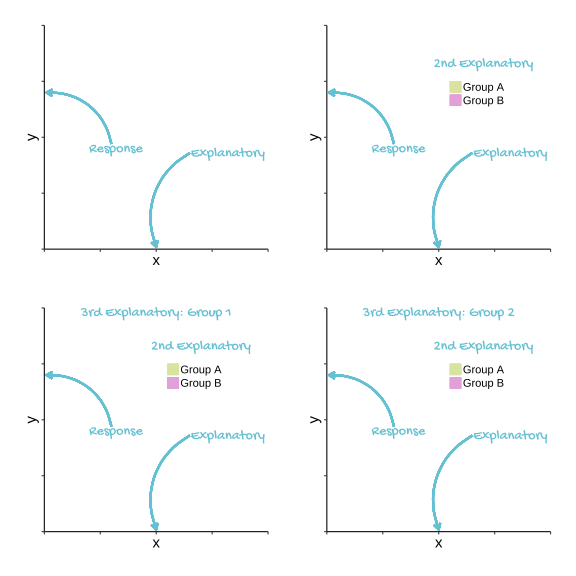
\includegraphics[width=0.8\linewidth]{images/fig_1} \end{flushleft}

If we have two explanatory variables we might indicate the different values of one of them with colour.

\begin{flushleft}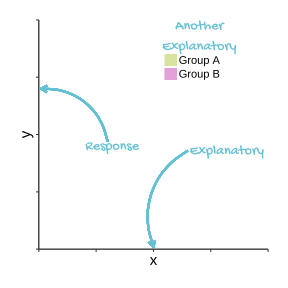
\includegraphics[width=0.8\linewidth]{images/fig_2} \end{flushleft}

In choosing between regression, \emph{t}-tests, one-way ANOVA and two-way ANOVA we consider how many explanatory variables we have and whether they are continuous or categorical. If we have one explanatory variable and it is continuous, we can apply a regression; if it is a categorical variable with two groups (or levels) we have the choice of a \emph{t}-test or a one way ANOVA but when there are more than two groups we use a one-way ANOVA. A two-way ANOVA is used when there are two categorical explanatory variables.

\begin{flushleft}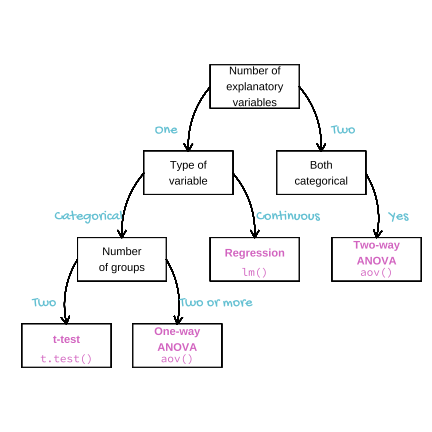
\includegraphics[width=1\linewidth]{images/fig_3} \end{flushleft}

These apparently different tests are, in fact, the same test. They have the same underlying mathematics and, or to put it another way, the follow the same model. That model is usually known as the \textbf{General Linear Model}.

Running a test = building or fitting a model. tests of how well our data fit the model, tests for the model parameters against a null hypothesis

In R \emph{t}-tests and ANOVA, like regression, can be carried out with the \texttt{lm()} function. The output differs but the results themselves are identical. The model makes a prediction for the response variable for a given value of the explanatory variable. The difference between the predicted value and the observed value is the residual.

\begin{key}

\texttt{lm()} can be used to perform tests using the General Linear Model including \emph{t}-tests, ANOVA and regression for response variables which are normally distributed.

\end{key}

The General Linear Model requires that the response variable has residuals that follow the normal distribution with variance which is homogeneous for the values of the explanatory variables. This commonly occurs when the response variable has a normal distribution. The \textbf{General\_ised\_} Linear Model* extends the General Linear Model by including response variables that do not follow the normal distribution.

\hypertarget{what-are-linear-models}{%
\chapter{What are linear models}\label{what-are-linear-models}}

\hypertarget{what-is-a-linear-model}{%
\section{What is a linear model?}\label{what-is-a-linear-model}}

A linear model describes a continuous response variable as a function of one or more explanatory variables. When you have a single explanatory variable, that model is:

\begin{equation}
y_{i}=\beta_{0}+\beta_{1}X1_{i}+e_{i}
\label{eq:lm1}
\end{equation}

Where:

\begin{itemize}
\tightlist
\item
  The response variable is \(y\) and \(X1\) is the explanatory variable.\\
\item
  \(\beta_{0}\) and \(\beta_{1}\) are the coefficients in the model. In a single linear regression, \(\beta_{0}\) is often called the intercept and \(\beta_{1}\) the slope.\\
\item
  \(i\) is the index of the response so \(y_{i}\) is the \(i\)th response; if you had 20 pairs of \(x\)-\(y\) values, \(i\) would go from 1 to 20.\\
\item
  \(e_{i}\) is the ``error'' also known as the residual.
\end{itemize}

The equation means the response can be predicted from a given value of the explanatory variable, \(\beta_{0}\) and \(\beta_{1}\) and will take that value plus some random noise. When you build a linear model from your data the procedure estimates the model coefficients.

See figure \ref{fig:lm-annotated}.



\begin{figure}

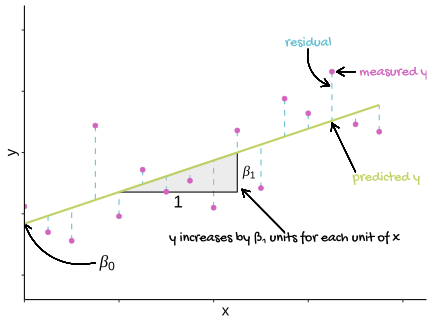
\includegraphics[width=0.8\linewidth]{images/fig_4} \hfill{}

\caption{Terms used in linear models. The measured \textcolor[HTML]{d264c0}{\textbf{response values are in pink}}, the \textcolor[HTML]{c0d264}{\textbf{predictions are in green}}, and the differences between these, known as the \textcolor[HTML]{64c0d2}{\textbf{residuals, are in blue}}. The estimated model parameters, \(\beta_{0}\) and \(\beta_{1}\) are indicated.}\label{fig:lm-annotated}
\end{figure}

\textbf{keypoint}
terminology build fit
parameter, coefficient
estimates

If you have more than one explanatory variable this these are given as \(X2\), \(X3\) and so on up to the \(p\)th explanatory variable each with its own \(\beta\) coefficient. The general form of the model is:
\begin{equation}
y_{i}=\beta_{0}+\beta_{1}X1_{i}+\beta_{2}X2_{i}+...+\beta_{p}XP_{i}+e_{i}
\label{eq:regression}
\end{equation}

\hypertarget{single-linear-regression}{%
\chapter{Single linear regression}\label{single-linear-regression}}

\hypertarget{introduction-to-the-example}{%
\section{Introduction to the example}\label{introduction-to-the-example}}

This is a test you have probably carried out before.

The concentration of juvenile hormone in stag beetles (\emph{Lucanus cervus}) is known to influence mandible growth. Groups of stag beetles were injected with different concentrations of juvenile hormone (pg\(\mu\)l\textsuperscript{-1}) and their average mandible size (mm) determined. The data are in \href{data-raw/stag.txt}{stag.txt}.

We will import the data with the \texttt{read\_table2()} function from the \texttt{readr} package and plot it with \texttt{ggplot()} from the \texttt{ggplot2} package. Both packages are part of the tidyverse and we load this first:

\begin{Shaded}
\begin{Highlighting}[]
\KeywordTok{library}\NormalTok{(tidyverse)}
\end{Highlighting}
\end{Shaded}

\begin{Shaded}
\begin{Highlighting}[]
\NormalTok{stag <-}\StringTok{ }\KeywordTok{read_table2}\NormalTok{(}\StringTok{"data-raw/stag.txt"}\NormalTok{)}
\end{Highlighting}
\end{Shaded}

Juvenile hormone is has been set by the experimenter and mandible size has decimal places and is something we would expect to be normally distributed. Visualising our data before any further analysis is usually sensible. In this case, it will help us determine if any relationship between the two variables is linear.

\begin{Shaded}
\begin{Highlighting}[]
\KeywordTok{ggplot}\NormalTok{(}\DataTypeTok{data =}\NormalTok{ stag, }\KeywordTok{aes}\NormalTok{(}\DataTypeTok{x =}\NormalTok{ jh, }\DataTypeTok{y =}\NormalTok{ mand)) }\OperatorTok{+}
\StringTok{        }\KeywordTok{geom_point}\NormalTok{()}
\end{Highlighting}
\end{Shaded}

\begin{flushleft}\includegraphics[width=0.8\linewidth]{single_linear_regression_files/figure-latex/unnamed-chunk-3-1} \end{flushleft}

The relationship between them looks roughly linear. So far, common sense suggests the assumptions of regression are met.

\hypertarget{applying-and-interpreting-lm}{%
\section{\texorpdfstring{Applying and interpreting \texttt{lm()}}{Applying and interpreting lm()}}\label{applying-and-interpreting-lm}}

The \texttt{lm()} function is used to build the regression model

\begin{Shaded}
\begin{Highlighting}[]
\CommentTok{# build the statistical model}
\NormalTok{mod <-}\StringTok{ }\KeywordTok{lm}\NormalTok{(}\DataTypeTok{data =}\NormalTok{ stag, mand }\OperatorTok{~}\StringTok{ }\NormalTok{jh)}
\end{Highlighting}
\end{Shaded}

This can be read as: fit a linear of model of mandible size explained by juvenile growth hormone concentration.

Printing \texttt{mod} to the console will reveal the estimated model parameters (coefficients) but little else:

\begin{Shaded}
\begin{Highlighting}[]
\NormalTok{mod}
\CommentTok{# }
\CommentTok{# Call:}
\CommentTok{# lm(formula = mand ~ jh, data = stag)}
\CommentTok{# }
\CommentTok{# Coefficients:}
\CommentTok{# (Intercept)           jh  }
\CommentTok{#     0.41934      0.00646}
\end{Highlighting}
\end{Shaded}

\(\beta_{0}\) is labelled ``(Intercept)'' and \(\beta_{1}\) is labelled ``jh''. Thus the equation of the line is:

\(mand\) = 0.419 + 0.006\(jh\)

More information including statistical tests of the model and its parameters is obtained by using \texttt{summary()}

\begin{Shaded}
\begin{Highlighting}[]
\CommentTok{# examine it}
\KeywordTok{summary}\NormalTok{(mod)}
\CommentTok{# }
\CommentTok{# Call:}
\CommentTok{# lm(formula = mand ~ jh, data = stag)}
\CommentTok{# }
\CommentTok{# Residuals:}
\CommentTok{#     Min      1Q  Median      3Q     Max }
\CommentTok{# -0.3860 -0.2028 -0.0975  0.1503  0.6069 }
\CommentTok{# }
\CommentTok{# Coefficients:}
\CommentTok{#             Estimate Std. Error t value Pr(>|t|)   }
\CommentTok{# (Intercept)  0.41934    0.13943    3.01   0.0094 **}
\CommentTok{# jh           0.00646    0.00158    4.08   0.0011 **}
\CommentTok{# ---}
\CommentTok{# Signif. codes:  0 '***' 0.001 '**' 0.01 '*' 0.05 '.' 0.1 ' ' 1}
\CommentTok{# }
\CommentTok{# Residual standard error: 0.292 on 14 degrees of freedom}
\CommentTok{# Multiple R-squared:  0.543,   Adjusted R-squared:  0.51 }
\CommentTok{# F-statistic: 16.6 on 1 and 14 DF,  p-value: 0.00113}
\end{Highlighting}
\end{Shaded}

The ``Coefficients:'' table gives the estimated \(\beta_{0}\) and \(\beta_{1}\) again, this time with their standard errors and tests of whether the estimates differ from zero. The estimated value for the intercept is 0.419 \(\pm\) 0.139 and this differs significantly from zero (\(p\) = 0.009). The estimated value for the slope, 0.006 \(\pm\) 0.002, also differs significantly from zero (\(p\) = 0.001).

The three lines at the bottom of the output gives information about the fit of the model to the data. The ``Multiple R-squared'' gives the proportion of the variance in the response which is explained by the model. In our case, 0.543 of the variance in mandible length is explained by the model and this is a significant proportion of that variance (\(p\) = 0.001).

For a single linear regression, the \emph{p}-value for the model and the \emph{p}-value for the slope are the same. This is also true for linear models in the form of a two-sample \emph{t}-test but \textbf{not} the case for other linear models.

\hypertarget{getting-predictions-from-the-model}{%
\section{Getting predictions from the model}\label{getting-predictions-from-the-model}}

The \texttt{predict()} returns the predicted values of the response. To add a column of predicted values to the dataframe:

\begin{Shaded}
\begin{Highlighting}[]
\NormalTok{stag}\OperatorTok{$}\NormalTok{pred <-}\StringTok{ }\KeywordTok{predict}\NormalTok{(mod)}
\end{Highlighting}
\end{Shaded}

This requires creating a data frame of the x values from which you want to predict

\begin{Shaded}
\begin{Highlighting}[]
\NormalTok{predictions <-}\StringTok{ }\KeywordTok{data.frame}\NormalTok{(}\DataTypeTok{jh =} \KeywordTok{seq}\NormalTok{(}\DecValTok{0}\NormalTok{, }\DecValTok{150}\NormalTok{, }\DecValTok{5}\NormalTok{))}
\end{Highlighting}
\end{Shaded}

Note that the name and type of value of explanatory variable must be the same as it is in the model

\begin{Shaded}
\begin{Highlighting}[]
\NormalTok{predictions}\OperatorTok{$}\NormalTok{pred <-}\StringTok{ }\KeywordTok{predict}\NormalTok{(mod, }\DataTypeTok{newdata =}\NormalTok{ predictions)}
\end{Highlighting}
\end{Shaded}

Replacing the terms shown in Figure \ref{fig:lm-annotated} with the values in this example gives us \ref{fig:stag-annotated}.



\begin{figure}

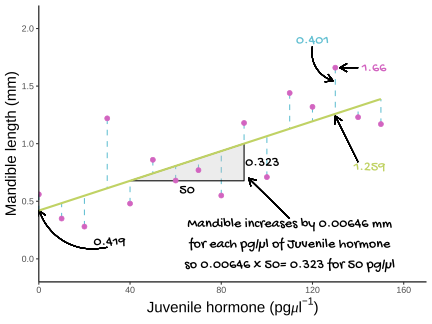
\includegraphics[width=0.8\linewidth]{images/fig_5} \hfill{}

\caption{these model estimates.}\label{fig:stag-annotated}
\end{figure}

\hypertarget{checking-assumptions}{%
\section{Checking assumptions}\label{checking-assumptions}}

\begin{Shaded}
\begin{Highlighting}[]
\KeywordTok{plot}\NormalTok{(mod, }\DataTypeTok{which =} \DecValTok{2}\NormalTok{)}
\KeywordTok{plot}\NormalTok{(mod, }\DataTypeTok{which =} \DecValTok{1}\NormalTok{)}
\KeywordTok{shapiro.test}\NormalTok{(mod}\OperatorTok{$}\NormalTok{res)}
\CommentTok{# }
\CommentTok{#   Shapiro-Wilk normality test}
\CommentTok{# }
\CommentTok{# data:  mod$res}
\CommentTok{# W = 0.9, p-value = 0.4}
\end{Highlighting}
\end{Shaded}

\begin{flushleft}\includegraphics[width=0.8\linewidth]{single_linear_regression_files/figure-latex/unnamed-chunk-11-1} \includegraphics[width=0.8\linewidth]{single_linear_regression_files/figure-latex/unnamed-chunk-11-2} \end{flushleft}

\hypertarget{creating-a-figure}{%
\section{Creating a figure}\label{creating-a-figure}}

\begin{Shaded}
\begin{Highlighting}[]
\KeywordTok{ggplot}\NormalTok{(}\DataTypeTok{data =}\NormalTok{ stag, }\KeywordTok{aes}\NormalTok{(}\DataTypeTok{x =}\NormalTok{ jh, }\DataTypeTok{y =}\NormalTok{ mand)) }\OperatorTok{+}
\StringTok{        }\KeywordTok{geom_point}\NormalTok{() }\OperatorTok{+}
\StringTok{        }\KeywordTok{scale_x_continuous}\NormalTok{(}\DataTypeTok{expand =} \KeywordTok{c}\NormalTok{(}\FloatTok{0.01}\NormalTok{, }\DecValTok{0}\NormalTok{),}
                           \DataTypeTok{limits =} \KeywordTok{c}\NormalTok{(}\DecValTok{0}\NormalTok{, }\DecValTok{160}\NormalTok{),}
                           \DataTypeTok{name =} \KeywordTok{expression}\NormalTok{(}\KeywordTok{paste}\NormalTok{(}\StringTok{"Juvenile hormone (pg"}\NormalTok{,}
\NormalTok{                                                   mu,}
\NormalTok{                                                   l}\OperatorTok{^-}\DecValTok{1}\NormalTok{,}
                                                   \StringTok{")"}\NormalTok{))) }\OperatorTok{+}
\StringTok{        }\KeywordTok{scale_y_continuous}\NormalTok{(}\DataTypeTok{expand =} \KeywordTok{c}\NormalTok{(}\DecValTok{0}\NormalTok{, }\DecValTok{0}\NormalTok{),}
                           \DataTypeTok{limits =} \KeywordTok{c}\NormalTok{(}\DecValTok{0}\NormalTok{, }\DecValTok{2}\NormalTok{),}
                           \DataTypeTok{name =} \StringTok{"Mandible length (mm)"}\NormalTok{) }\OperatorTok{+}
\StringTok{        }\KeywordTok{geom_smooth}\NormalTok{(}\DataTypeTok{method =}\NormalTok{ lm, }\DataTypeTok{se =} \OtherTok{FALSE}\NormalTok{, }\DataTypeTok{colour =} \StringTok{"black"}\NormalTok{) }\OperatorTok{+}
\StringTok{        }\KeywordTok{theme_classic}\NormalTok{()}
\end{Highlighting}
\end{Shaded}

\begin{flushleft}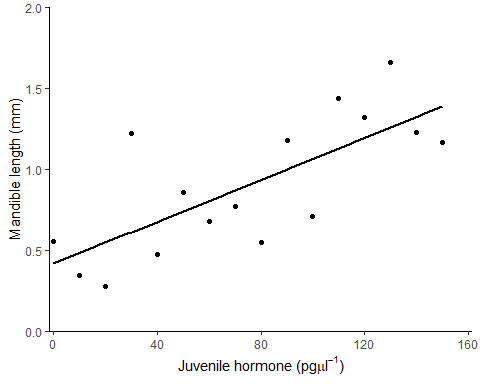
\includegraphics[width=0.8\linewidth]{single_linear_regression_files/figure-latex/fig-reg-1} \end{flushleft}

\hypertarget{reporting-the-results}{%
\section{Reporting the results}\label{reporting-the-results}}

There was a significant positive relationship between the concentration of Juvenile hormone and mandible length (\(\beta_{1}\pm s.e.\): 0.006 \(\pm\) 0.002; \(p\) = 0.001). See figure \ref{fig:fig-reg-report}.



\begin{figure}

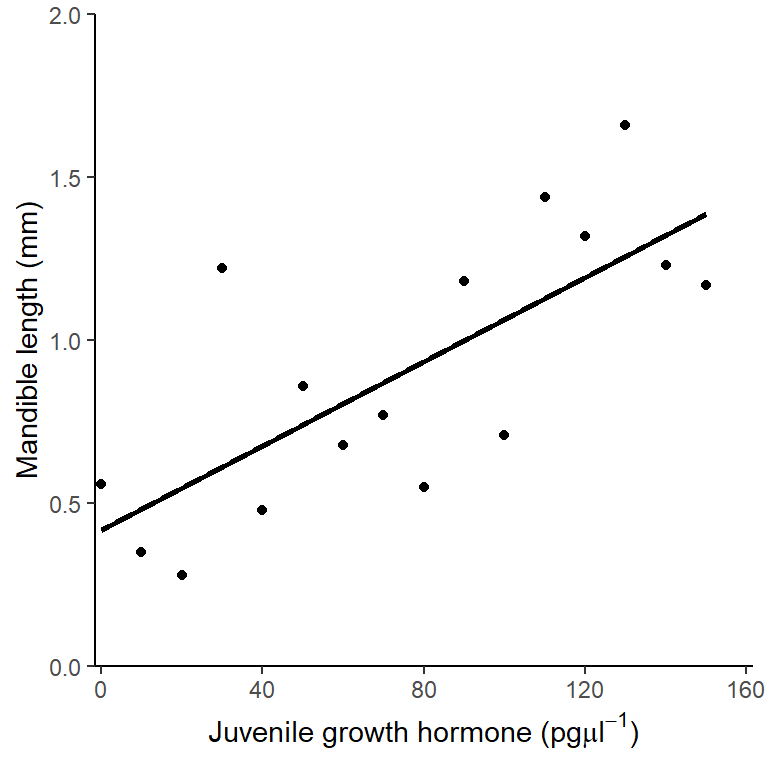
\includegraphics[width=0.8\linewidth]{single_linear_regression_files/figure-latex/fig-reg-report-1} \hfill{}

\caption{Relationship between the concentration of Juvenile hormone and mandible length.}\label{fig:fig-reg-report}
\end{figure}

\hypertarget{part-using-lm-for-familiar-tests}{%
\part{Using 'lm()` for familiar tests}\label{part-using-lm-for-familiar-tests}}

\hypertarget{t-tests-revisit}{%
\chapter{\texorpdfstring{\emph{t}-tests revisited}{t-tests revisited}}\label{t-tests-revisit}}

\hypertarget{introduction-to-the-example-1}{%
\section{Introduction to the example}\label{introduction-to-the-example-1}}

Some plant biotechnologists developed a genetically modified line of \emph{Cannabis sativa} to increase its omega 3 fatty acids content. They grew 50 wild type and fifty modified plants to maturity, collect the seeds and measure the amount of omega 3 fatty acids. The data are in \href{data-raw/csativa.txt}{csativa.txt}. They used a two-sample \emph{t}-test to compare the mean omega 3 content in the two plant types.

We again use the \texttt{read\_table2()} function to import the data and visualise it with \texttt{ggplot()}

\begin{Shaded}
\begin{Highlighting}[]
\KeywordTok{library}\NormalTok{(tidyverse)}
\end{Highlighting}
\end{Shaded}

\begin{Shaded}
\begin{Highlighting}[]
\NormalTok{csativa  <-}\StringTok{  }\KeywordTok{read_table2}\NormalTok{(}\StringTok{"data-raw/csativa.txt"}\NormalTok{)}
\end{Highlighting}
\end{Shaded}

\begin{Shaded}
\begin{Highlighting}[]
\CommentTok{# create a rough plot of the data  }
\KeywordTok{ggplot}\NormalTok{(}\DataTypeTok{data =}\NormalTok{ csativa, }\KeywordTok{aes}\NormalTok{(}\DataTypeTok{x =}\NormalTok{ plant, }\DataTypeTok{y =}\NormalTok{ omega)) }\OperatorTok{+}
\StringTok{  }\KeywordTok{geom_violin}\NormalTok{()}
\end{Highlighting}
\end{Shaded}

\begin{flushleft}\includegraphics[width=0.8\linewidth]{t_test_revisit_files/figure-latex/unnamed-chunk-3-1} \end{flushleft}

The modified plant have a lower mean omega 3 content than the wildtype plants. The modification appears not to be successful.

Statistical comparison of the two means can be done with either the \texttt{t.test()} or \texttt{lm()} functions; these are exactly equivalent but present the results differently. We will use our understanding of applying and interpreting \texttt{t.test()} to develop our understanding of \texttt{lm()} output

\hypertarget{t.test-output-reminder}{%
\section{\texorpdfstring{\texttt{t.test()} output reminder}{t.test() output reminder}}\label{t.test-output-reminder}}

\begin{Shaded}
\begin{Highlighting}[]
\KeywordTok{t.test}\NormalTok{(}\DataTypeTok{data =}\NormalTok{ csativa, omega }\OperatorTok{~}\StringTok{ }\NormalTok{plant, }\DataTypeTok{var.equal =} \OtherTok{TRUE}\NormalTok{)}
\CommentTok{# }
\CommentTok{#   Two Sample t-test}
\CommentTok{# }
\CommentTok{# data:  omega by plant}
\CommentTok{# t = -5, df = 98, p-value = 2e-06}
\CommentTok{# alternative hypothesis: true difference in means is not equal to 0}
\CommentTok{# 95 percent confidence interval:}
\CommentTok{#  -9.69 -4.21}
\CommentTok{# sample estimates:}
\CommentTok{# mean in group modif  mean in group wild }
\CommentTok{#                49.5                56.4}
\end{Highlighting}
\end{Shaded}

The two groups means are give in the section labelled ``sample estimates'' and the test of whether they differ significantly is given in the forth line (beginning ``t = \ldots{}''). We conclude the mean omega 3 content of the modified plants (49.465) is significantly lower than that of the wildtype plants (\(t\) = 5.029, \(d.f.\) = 98, \(p\) = \ensuremath{2.231\times 10^{-6}}).

The confidence interval is on the difference between the two means.

The sign on the \(t\) value and the order in which the sample estimates are given is determined by R's alphabetical ordering of the groups. As ``modif'' comes before ``wildtype'' in the alphabet, ``modif'' is the first group and the test is the modified plant mean minus the wildtype mean. This has no impact on our conclusions and had the wildtype plants been labelled ``control'' the output would be:

\begin{verbatim}
    Two Sample t-test

data:  omega by plant
t = 5.0289, df = 98, p-value = 2.231e-06
alternative hypothesis: true difference in means is not equal to 0
95 percent confidence interval:
 4.205372 9.687828
sample estimates:
mean in group control  mean in group modif
            56.4118             49.4652
\end{verbatim}

\hypertarget{applying-and-interpreting-lm-1}{%
\section{\texorpdfstring{Applying and interpreting \texttt{lm()}}{Applying and interpreting lm()}}\label{applying-and-interpreting-lm-1}}

The \texttt{lm()} function is used as follows:

\begin{Shaded}
\begin{Highlighting}[]
\CommentTok{# build a model with `lm()`}
\NormalTok{mod <-}\StringTok{ }\KeywordTok{lm}\NormalTok{(omega }\OperatorTok{~}\StringTok{ }\NormalTok{plant, }\DataTypeTok{data =}\NormalTok{ csativa)}
\end{Highlighting}
\end{Shaded}

This can be read as: fit a linear of model of omega content explained by plant type. Printing \texttt{mod} to the console gives us these estimated model parameters (coefficients):

\begin{Shaded}
\begin{Highlighting}[]
\NormalTok{mod}
\CommentTok{# }
\CommentTok{# Call:}
\CommentTok{# lm(formula = omega ~ plant, data = csativa)}
\CommentTok{# }
\CommentTok{# Coefficients:}
\CommentTok{# (Intercept)    plantwild  }
\CommentTok{#       49.47         6.95}
\end{Highlighting}
\end{Shaded}

\begin{Shaded}
\begin{Highlighting}[]
\KeywordTok{summary}\NormalTok{(mod)}
\CommentTok{# }
\CommentTok{# Call:}
\CommentTok{# lm(formula = omega ~ plant, data = csativa)}
\CommentTok{# }
\CommentTok{# Residuals:}
\CommentTok{#     Min      1Q  Median      3Q     Max }
\CommentTok{# -15.872  -3.703  -0.964   4.460  16.918 }
\CommentTok{# }
\CommentTok{# Coefficients:}
\CommentTok{#             Estimate Std. Error t value Pr(>|t|)    }
\CommentTok{# (Intercept)   49.465      0.977   50.64  < 2e-16 ***}
\CommentTok{# plantwild      6.947      1.381    5.03  2.2e-06 ***}
\CommentTok{# ---}
\CommentTok{# Signif. codes:  0 '***' 0.001 '**' 0.01 '*' 0.05 '.' 0.1 ' ' 1}
\CommentTok{# }
\CommentTok{# Residual standard error: 6.91 on 98 degrees of freedom}
\CommentTok{# Multiple R-squared:  0.205,   Adjusted R-squared:  0.197 }
\CommentTok{# F-statistic: 25.3 on 1 and 98 DF,  p-value: 2.23e-06}
\end{Highlighting}
\end{Shaded}

\hypertarget{getting-predictions-from-the-model-1}{%
\section{Getting predictions from the model}\label{getting-predictions-from-the-model-1}}

\begin{Shaded}
\begin{Highlighting}[]
\NormalTok{predictions <-}\StringTok{ }\KeywordTok{data.frame}\NormalTok{(}\DataTypeTok{plant =} \KeywordTok{c}\NormalTok{(}\StringTok{"modif"}\NormalTok{, }\StringTok{"wild"}\NormalTok{))}
\end{Highlighting}
\end{Shaded}

\begin{Shaded}
\begin{Highlighting}[]
\NormalTok{predictions}\OperatorTok{$}\NormalTok{pred <-}\StringTok{ }\KeywordTok{predict}\NormalTok{(mod, }\DataTypeTok{newdata =}\NormalTok{ predictions)}
\end{Highlighting}
\end{Shaded}

Replacing the terms shown in Figure \ref{fig:lm-annotated} with the values in this example gives us \ref{fig:csat-annotated}.



\begin{figure}

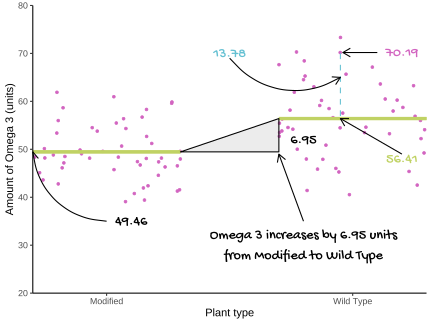
\includegraphics[width=0.8\linewidth]{images/fig_6} \hfill{}

\caption{these model estimates.}\label{fig:csat-annotated}
\end{figure}

\hypertarget{checking-assumptions-1}{%
\section{Checking assumptions}\label{checking-assumptions-1}}

\begin{Shaded}
\begin{Highlighting}[]
\KeywordTok{plot}\NormalTok{(mod, }\DataTypeTok{which =} \DecValTok{2}\NormalTok{)}
\KeywordTok{plot}\NormalTok{(mod, }\DataTypeTok{which =} \DecValTok{1}\NormalTok{)}
\KeywordTok{shapiro.test}\NormalTok{(mod}\OperatorTok{$}\NormalTok{res)}
\CommentTok{# }
\CommentTok{#   Shapiro-Wilk normality test}
\CommentTok{# }
\CommentTok{# data:  mod$res}
\CommentTok{# W = 1, p-value = 0.5}
\end{Highlighting}
\end{Shaded}

\begin{flushleft}\includegraphics[width=0.8\linewidth]{t_test_revisit_files/figure-latex/unnamed-chunk-11-1} \includegraphics[width=0.8\linewidth]{t_test_revisit_files/figure-latex/unnamed-chunk-11-2} \end{flushleft}

\hypertarget{creating-a-figure-1}{%
\section{Creating a figure}\label{creating-a-figure-1}}

\begin{Shaded}
\begin{Highlighting}[]
\NormalTok{csativa_summary <-}\StringTok{ }\NormalTok{csativa }\OperatorTok
\StringTok{  }\KeywordTok{group_by}\NormalTok{(plant) }\OperatorTok
\StringTok{  }\KeywordTok{summarise}\NormalTok{(}\DataTypeTok{mean =} \KeywordTok{mean}\NormalTok{(omega),}
            \DataTypeTok{std =} \KeywordTok{sd}\NormalTok{(omega),}
            \DataTypeTok{n =} \KeywordTok{length}\NormalTok{(omega),}
            \DataTypeTok{se =}\NormalTok{ std}\OperatorTok{/}\KeywordTok{sqrt}\NormalTok{(n))}
\end{Highlighting}
\end{Shaded}

\begin{Shaded}
\begin{Highlighting}[]
\CommentTok{#summarise the data }

\KeywordTok{ggplot}\NormalTok{() }\OperatorTok{+}
\StringTok{  }\KeywordTok{geom_jitter}\NormalTok{(}\DataTypeTok{data =}\NormalTok{ csativa, }
              \KeywordTok{aes}\NormalTok{(}\DataTypeTok{x =}\NormalTok{ plant, }\DataTypeTok{y =}\NormalTok{ omega), }
              \DataTypeTok{width =} \FloatTok{0.25}\NormalTok{, }\DataTypeTok{colour =} \StringTok{"grey"}\NormalTok{) }\OperatorTok{+}
\StringTok{  }\KeywordTok{geom_errorbar}\NormalTok{(}\DataTypeTok{data =}\NormalTok{ csativa_summary,}
                \KeywordTok{aes}\NormalTok{(}\DataTypeTok{x =}\NormalTok{ plant,}
                    \DataTypeTok{ymin =}\NormalTok{ mean,}
                    \DataTypeTok{ymax =}\NormalTok{ mean),}
                \DataTypeTok{width =} \FloatTok{.3}\NormalTok{) }\OperatorTok{+}
\StringTok{  }\KeywordTok{geom_errorbar}\NormalTok{(}\DataTypeTok{data =}\NormalTok{ csativa_summary,}
                \KeywordTok{aes}\NormalTok{(}\DataTypeTok{x =}\NormalTok{ plant,}
                    \DataTypeTok{ymin =}\NormalTok{ mean }\OperatorTok{-}\StringTok{ }\NormalTok{se,}
                    \DataTypeTok{ymax =}\NormalTok{ mean }\OperatorTok{+}\StringTok{ }\NormalTok{se),}
                \DataTypeTok{width =} \FloatTok{.5}\NormalTok{) }\OperatorTok{+}
\StringTok{  }\KeywordTok{geom_segment}\NormalTok{(}\KeywordTok{aes}\NormalTok{(}\DataTypeTok{x =} \DecValTok{1}\NormalTok{, }\DataTypeTok{y =} \DecValTok{75}\NormalTok{, }\DataTypeTok{xend =} \DecValTok{2}\NormalTok{, }\DataTypeTok{yend =} \DecValTok{75}\NormalTok{),}
               \DataTypeTok{size =} \DecValTok{1}\NormalTok{) }\OperatorTok{+}
\StringTok{  }\KeywordTok{geom_segment}\NormalTok{(}\KeywordTok{aes}\NormalTok{(}\DataTypeTok{x =} \DecValTok{1}\NormalTok{, }\DataTypeTok{y =} \DecValTok{75}\NormalTok{, }\DataTypeTok{xend =} \DecValTok{1}\NormalTok{, }\DataTypeTok{yend =} \DecValTok{73}\NormalTok{),}
               \DataTypeTok{size =} \DecValTok{1}\NormalTok{) }\OperatorTok{+}
\StringTok{  }\KeywordTok{geom_segment}\NormalTok{(}\KeywordTok{aes}\NormalTok{(}\DataTypeTok{x =} \DecValTok{2}\NormalTok{, }\DataTypeTok{y =} \DecValTok{75}\NormalTok{, }\DataTypeTok{xend =} \DecValTok{2}\NormalTok{, }\DataTypeTok{yend =} \DecValTok{73}\NormalTok{),}
               \DataTypeTok{size =} \DecValTok{1}\NormalTok{) }\OperatorTok{+}
\StringTok{  }\KeywordTok{annotate}\NormalTok{(}\StringTok{"text"}\NormalTok{, }\DataTypeTok{x =} \FloatTok{1.5}\NormalTok{, }\DataTypeTok{y =} \DecValTok{77}\NormalTok{,  }\DataTypeTok{label =} \StringTok{"***"}\NormalTok{, }\DataTypeTok{size =} \DecValTok{6}\NormalTok{) }\OperatorTok{+}
\StringTok{  }\KeywordTok{scale_x_discrete}\NormalTok{(}\DataTypeTok{labels =} \KeywordTok{c}\NormalTok{(}\StringTok{"Modified"}\NormalTok{, }\StringTok{"Wild Type"}\NormalTok{),}
                   \DataTypeTok{name =} \StringTok{"Plant type"}\NormalTok{) }\OperatorTok{+}
\StringTok{  }\KeywordTok{scale_y_continuous}\NormalTok{(}\DataTypeTok{name =} \StringTok{"Amount of Omega 3 (units)"}\NormalTok{,}
                     \DataTypeTok{expand =} \KeywordTok{c}\NormalTok{(}\DecValTok{0}\NormalTok{, }\DecValTok{0}\NormalTok{),}
                     \DataTypeTok{limits =} \KeywordTok{c}\NormalTok{(}\DecValTok{0}\NormalTok{, }\DecValTok{90}\NormalTok{)) }\OperatorTok{+}
\StringTok{  }\KeywordTok{theme_classic}\NormalTok{()}
\end{Highlighting}
\end{Shaded}

\begin{flushleft}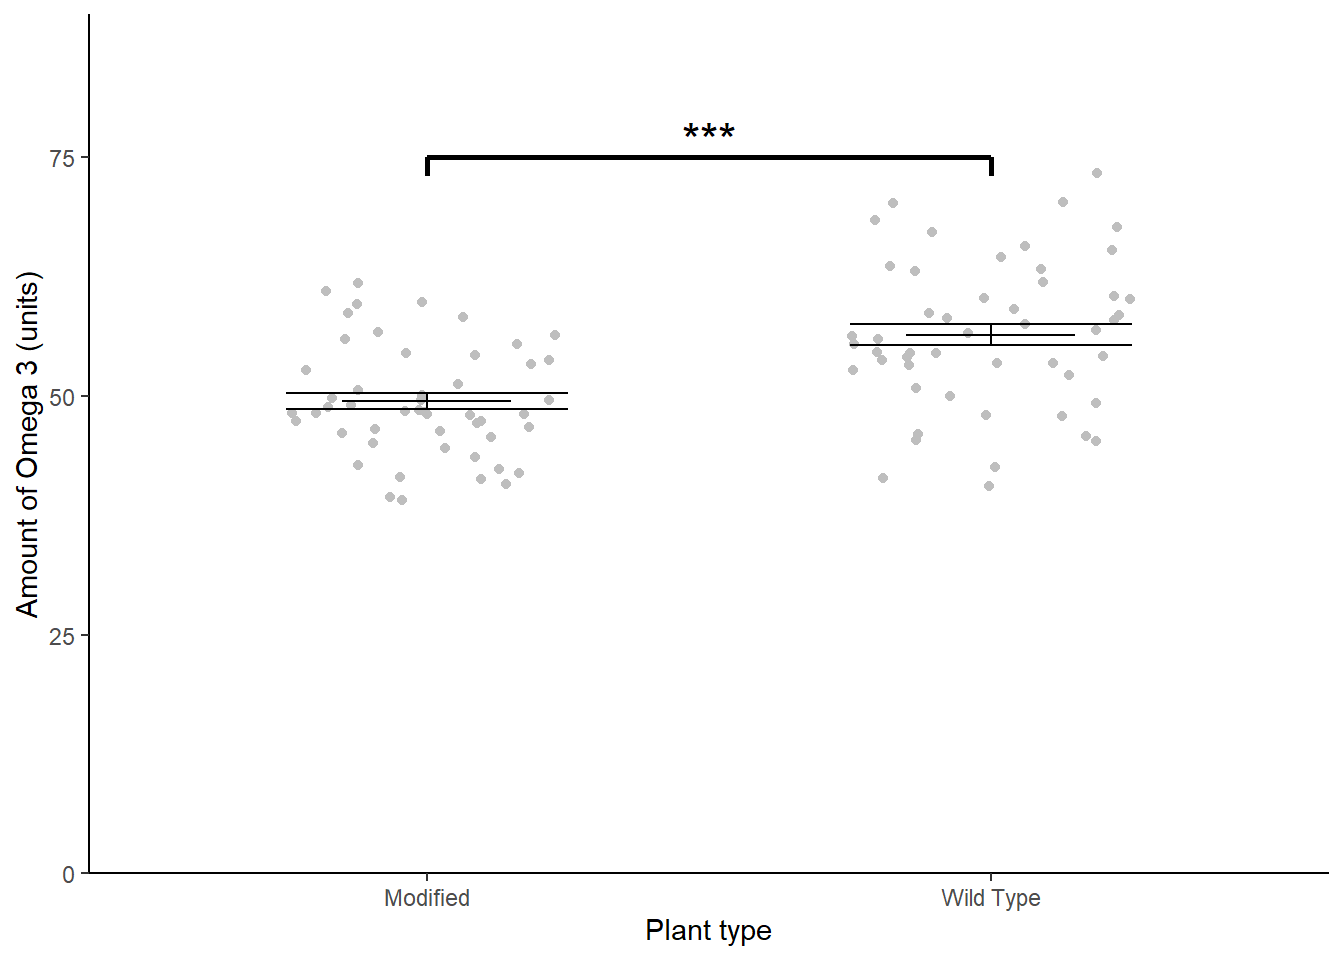
\includegraphics[width=0.8\linewidth]{t_test_revisit_files/figure-latex/fig-ttest-1} \end{flushleft}

\hypertarget{reporting-the-results-1}{%
\section{Reporting the results}\label{reporting-the-results-1}}

\begin{Shaded}
\begin{Highlighting}[]
\NormalTok{res <-}\StringTok{ }\KeywordTok{summary}\NormalTok{(mod)}
\NormalTok{tval <-}\StringTok{ }\NormalTok{res}\OperatorTok{$}\NormalTok{coefficients[}\StringTok{"plantwild"}\NormalTok{, }\StringTok{"t value"}\NormalTok{]}
\NormalTok{df <-}\StringTok{ }\NormalTok{res}\OperatorTok{$}\NormalTok{df[}\DecValTok{2}\NormalTok{]}
\end{Highlighting}
\end{Shaded}

The genetic modification was unsuccessful with wild type plants (\(\bar{x} \pm s.e.\): 56.4118 \(\pm\) 1.10968871126923) have significantly higher omega 3 than modified plants(49.4652 \(\pm\) 0.822615799924676) (\(t\) = 5.029; \(d.f.\) = 98; \(p\) \textless{} 0.001). See figure \ref{fig:fig-ttest-report}.



\begin{figure}

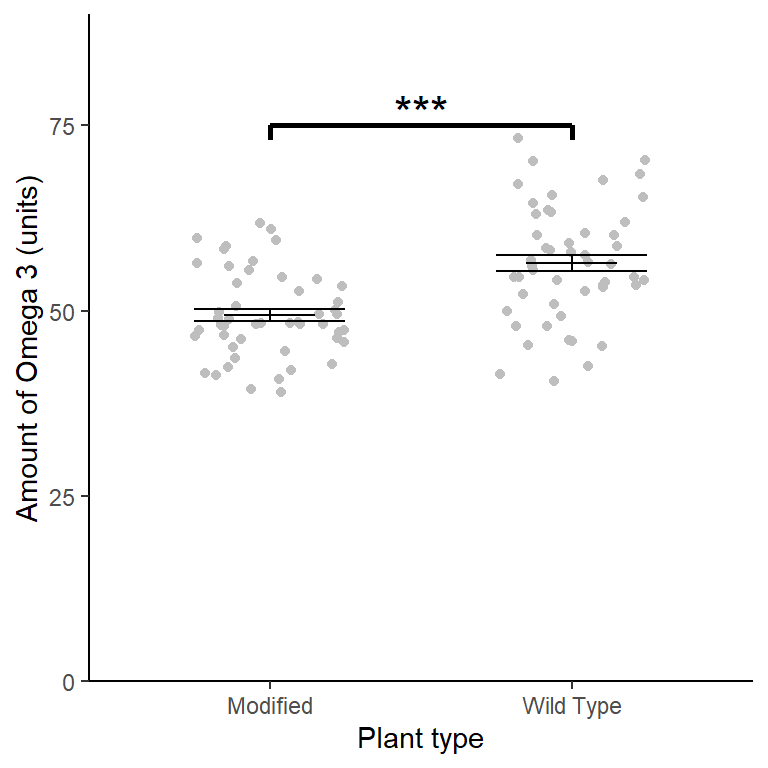
\includegraphics[width=0.8\linewidth]{t_test_revisit_files/figure-latex/fig-ttest-report-1} \hfill{}

\caption{Relationship between the concentration of Juvenile hormone and mandible length.}\label{fig:fig-ttest-report}
\end{figure}

\hypertarget{one-way-anova-revisit}{%
\chapter{One-way ANOVA revisited}\label{one-way-anova-revisit}}

\hypertarget{introduction-to-the-example-2}{%
\section{Introduction to the example}\label{introduction-to-the-example-2}}

The myoglobin concentration of skeletal muscle of three species of seal in grams per kilogram of muscle was determined and the data are given in \href{data-raw/seal.text}{seal.txt}. We want to know if there is a difference in myoglobin concentration between species. Each row represents an individual seal.

Figure \ref{fig:weddell-fig}



\begin{Shaded}
\begin{Highlighting}[]
\NormalTok{knitr}\OperatorTok{::}\KeywordTok{include_graphics}\NormalTok{(}\StringTok{"images/Baby_Weddell_Seal.jpg"}\NormalTok{)}
\end{Highlighting}
\end{Shaded}

\begin{figure}

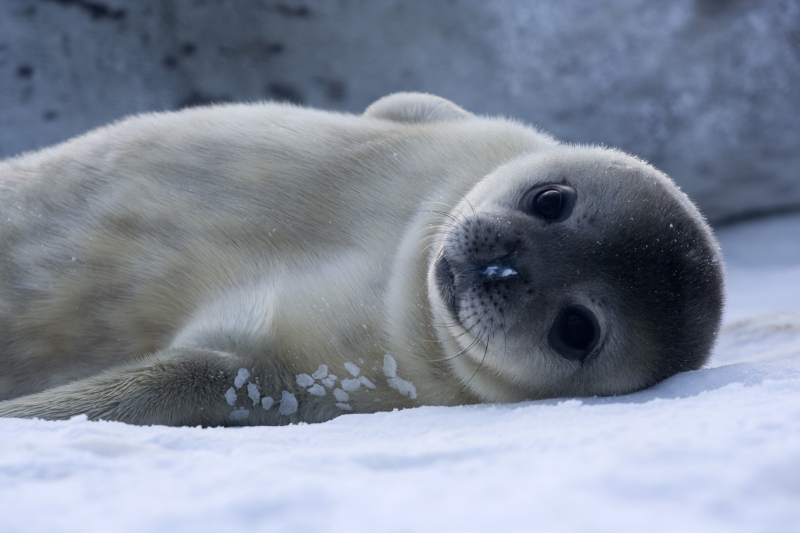
\includegraphics[width=0.8\linewidth,height=200px]{images/Baby_Weddell_Seal} \hfill{}

\caption{Baby Weddell Seals are very cute. By Photo © Samuel Blanc, CC BY-SA 3.0, \url{https://commons.wikimedia.org/w/index.php?curid=3877642}}\label{fig:weddell-fig}
\end{figure}

\begin{Shaded}
\begin{Highlighting}[]
\KeywordTok{library}\NormalTok{(tidyverse)}
\end{Highlighting}
\end{Shaded}

\begin{Shaded}
\begin{Highlighting}[]
\NormalTok{seal <-}\StringTok{ }\KeywordTok{read_delim}\NormalTok{(}\StringTok{"data-raw/seal.txt"}\NormalTok{, }\DataTypeTok{delim =} \StringTok{" "}\NormalTok{)}
\NormalTok{seal}\OperatorTok{$}\NormalTok{species <-}\StringTok{ }\KeywordTok{factor}\NormalTok{(seal}\OperatorTok{$}\NormalTok{species)}
\end{Highlighting}
\end{Shaded}

\begin{Shaded}
\begin{Highlighting}[]
\CommentTok{# create a rough plot of the data  }
\KeywordTok{ggplot}\NormalTok{(}\DataTypeTok{data =}\NormalTok{ seal, }\KeywordTok{aes}\NormalTok{(}\DataTypeTok{x =}\NormalTok{ species, }\DataTypeTok{y =}\NormalTok{ myoglobin)) }\OperatorTok{+}
\StringTok{  }\KeywordTok{geom_violin}\NormalTok{()}
\end{Highlighting}
\end{Shaded}

\begin{flushleft}\includegraphics[width=0.8\linewidth]{one_way_anova_revisit_files/figure-latex/unnamed-chunk-3-1} \end{flushleft}

\begin{Shaded}
\begin{Highlighting}[]
\NormalTok{seal_summary <-}\StringTok{ }\NormalTok{seal }\OperatorTok
\StringTok{  }\KeywordTok{group_by}\NormalTok{(species) }\OperatorTok
\StringTok{  }\KeywordTok{summarise}\NormalTok{(}\DataTypeTok{mean =} \KeywordTok{mean}\NormalTok{(myoglobin),}
            \DataTypeTok{std =} \KeywordTok{sd}\NormalTok{(myoglobin),}
            \DataTypeTok{n =} \KeywordTok{length}\NormalTok{(myoglobin),}
            \DataTypeTok{se =}\NormalTok{ std}\OperatorTok{/}\KeywordTok{sqrt}\NormalTok{(n))}
\end{Highlighting}
\end{Shaded}

\hypertarget{aov-output-reminder}{%
\section{\texorpdfstring{\texttt{aov} output reminder}{aov output reminder}}\label{aov-output-reminder}}

\begin{Shaded}
\begin{Highlighting}[]
\NormalTok{mod <-}\StringTok{ }\KeywordTok{aov}\NormalTok{(}\DataTypeTok{data =}\NormalTok{ seal, myoglobin }\OperatorTok{~}\StringTok{ }\NormalTok{species)}
\end{Highlighting}
\end{Shaded}

\begin{Shaded}
\begin{Highlighting}[]
\KeywordTok{summary}\NormalTok{(mod)}
\CommentTok{#             Df Sum Sq Mean Sq F value Pr(>F)   }
\CommentTok{# species      2    692     346    5.35 0.0064 **}
\CommentTok{# Residuals   87   5627      65                  }
\CommentTok{# ---}
\CommentTok{# Signif. codes:  0 '***' 0.001 '**' 0.01 '*' 0.05 '.' 0.1 ' ' 1}
\end{Highlighting}
\end{Shaded}

\begin{Shaded}
\begin{Highlighting}[]
\NormalTok{res <-}\StringTok{ }\KeywordTok{summary}\NormalTok{(mod)[[}\DecValTok{1}\NormalTok{]]}
\NormalTok{df1 <-}\StringTok{ }\NormalTok{res}\OperatorTok{$}\NormalTok{Df[}\DecValTok{1}\NormalTok{]}
\NormalTok{df2 <-}\StringTok{ }\NormalTok{res}\OperatorTok{$}\NormalTok{Df[}\DecValTok{2}\NormalTok{]}
\NormalTok{fval <-}\StringTok{ }\NormalTok{res}\OperatorTok{$}\StringTok{`}\DataTypeTok{F value}\StringTok{`}\NormalTok{[}\DecValTok{1}\NormalTok{]}
\NormalTok{pval <-}\StringTok{ }\NormalTok{res}\OperatorTok{$}\StringTok{`}\DataTypeTok{Pr(>F)}\StringTok{`}\NormalTok{[}\DecValTok{1}\NormalTok{]}
\end{Highlighting}
\end{Shaded}

\begin{Shaded}
\begin{Highlighting}[]
\KeywordTok{TukeyHSD}\NormalTok{(mod)}
\CommentTok{#   Tukey multiple comparisons of means}
\CommentTok{#     95% family-wise confidence level}
\CommentTok{# }
\CommentTok{# Fit: aov(formula = myoglobin ~ species, data = seal)}
\CommentTok{# }
\CommentTok{# $species}
\CommentTok{#                                diff   lwr    upr p adj}
\CommentTok{# Harbour Seal-Bladdernose Seal  6.69  1.74 11.646 0.005}
\CommentTok{# Weddell Seal-Bladdernose Seal  2.34 -2.61  7.296 0.499}
\CommentTok{# Weddell Seal-Harbour Seal     -4.35 -9.30  0.602 0.097}
\end{Highlighting}
\end{Shaded}

There is a significant difference in myoglobin concentration between Seal species (ANOVA: \(F\) = 5.352; \(d.f.\) = 2, 87; \$p \(= 0.006). Post-hoc testing revealed that difference to be between the Harbour Seal with the highest myoglobin concentrations (\)\bar\{x\} \pm s.e.\$: 49.0103333333333 \(\pm\) 1.50660289891503) ) and the Bladdernose Seal with the lowest (\(\bar{x} \pm s.e.\): 42.316 \(\pm\) 1.46436064272228).

\hypertarget{applying-and-interpreting-lm-2}{%
\section{\texorpdfstring{Applying and interpreting \texttt{lm()}}{Applying and interpreting lm()}}\label{applying-and-interpreting-lm-2}}

\begin{Shaded}
\begin{Highlighting}[]
\NormalTok{mod <-}\StringTok{ }\KeywordTok{lm}\NormalTok{(}\DataTypeTok{data =}\NormalTok{ seal, myoglobin }\OperatorTok{~}\StringTok{ }\NormalTok{species)}
\end{Highlighting}
\end{Shaded}

\begin{Shaded}
\begin{Highlighting}[]
\NormalTok{mod}
\CommentTok{# }
\CommentTok{# Call:}
\CommentTok{# lm(formula = myoglobin ~ species, data = seal)}
\CommentTok{# }
\CommentTok{# Coefficients:}
\CommentTok{#         (Intercept)  speciesHarbour Seal  speciesWeddell Seal  }
\CommentTok{#               42.32                 6.69                 2.34}
\end{Highlighting}
\end{Shaded}

\begin{Shaded}
\begin{Highlighting}[]
\NormalTok{coef <-}\StringTok{ }\NormalTok{mod}\OperatorTok{$}\NormalTok{coefficients}
\end{Highlighting}
\end{Shaded}

42.316
6.694
2.344

\hypertarget{getting-predictions-from-the-model-2}{%
\section{Getting predictions from the model}\label{getting-predictions-from-the-model-2}}

\begin{Shaded}
\begin{Highlighting}[]
\NormalTok{predictions <-}\StringTok{ }\KeywordTok{data.frame}\NormalTok{(}\DataTypeTok{species =}\NormalTok{ seal_summary}\OperatorTok{$}\NormalTok{species)}
\end{Highlighting}
\end{Shaded}

\begin{Shaded}
\begin{Highlighting}[]
\NormalTok{predictions}\OperatorTok{$}\NormalTok{pred <-}\StringTok{ }\KeywordTok{predict}\NormalTok{(mod, }\DataTypeTok{newdata =}\NormalTok{ predictions)}
\end{Highlighting}
\end{Shaded}

Replacing the terms shown in Figure \ref{fig:lm-annotated} with the values in this example gives us \ref{fig:one-way-annotated}.

(ref:fig:one-way-annotated) these model estimates.

\begin{figure}

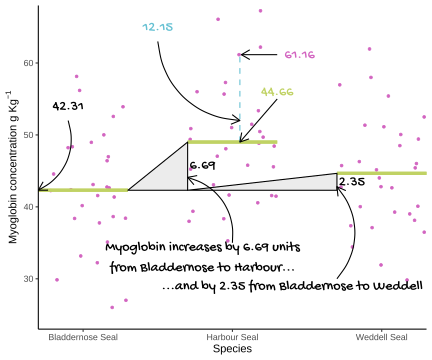
\includegraphics[width=0.8\linewidth]{images/fig_7} \hfill{}

\caption{(ref:one-way-annotated)}\label{fig:one-way-annotated}
\end{figure}

\hypertarget{checking-assumptions-2}{%
\section{Checking assumptions}\label{checking-assumptions-2}}

\begin{Shaded}
\begin{Highlighting}[]
\KeywordTok{plot}\NormalTok{(mod, }\DataTypeTok{which =} \DecValTok{2}\NormalTok{)}
\KeywordTok{plot}\NormalTok{(mod, }\DataTypeTok{which =} \DecValTok{1}\NormalTok{)}
\KeywordTok{shapiro.test}\NormalTok{(mod}\OperatorTok{$}\NormalTok{res)}
\CommentTok{# }
\CommentTok{#   Shapiro-Wilk normality test}
\CommentTok{# }
\CommentTok{# data:  mod$res}
\CommentTok{# W = 1, p-value = 0.4}
\end{Highlighting}
\end{Shaded}

\begin{flushleft}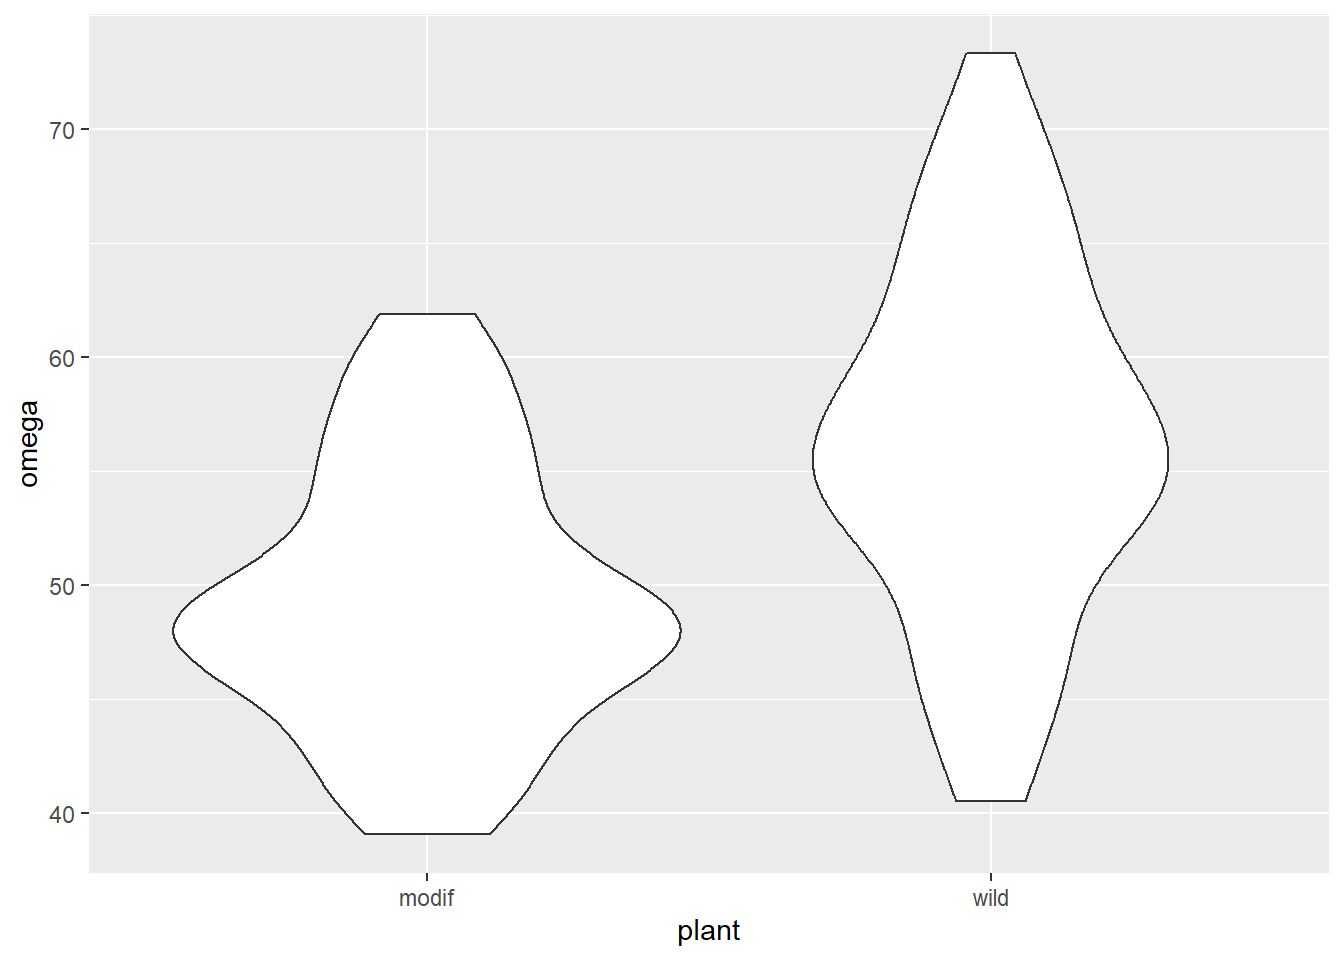
\includegraphics[width=0.8\linewidth]{one_way_anova_revisit_files/figure-latex/unnamed-chunk-14-1} 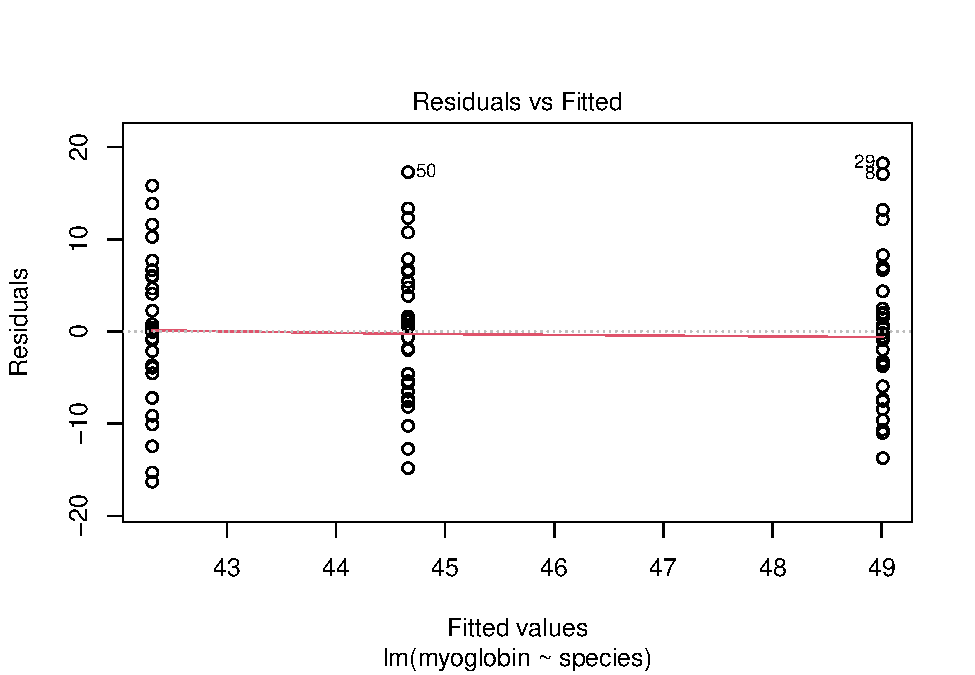
\includegraphics[width=0.8\linewidth]{one_way_anova_revisit_files/figure-latex/unnamed-chunk-14-2} \end{flushleft}

\begin{Shaded}
\begin{Highlighting}[]
\KeywordTok{library}\NormalTok{(multcomp)}
\end{Highlighting}
\end{Shaded}

\begin{Shaded}
\begin{Highlighting}[]
\NormalTok{mod_mc <-}\StringTok{ }\KeywordTok{glht}\NormalTok{(mod, }\DataTypeTok{linfct =} \KeywordTok{mcp}\NormalTok{(}\DataTypeTok{species =} \KeywordTok{c}\NormalTok{(}\StringTok{"`Bladdernose Seal` - `Harbour Seal` = 0"}\NormalTok{, }
                                             \StringTok{"`Bladdernose Seal` - `Weddell Seal` = 0"}\NormalTok{,}
                                             \StringTok{"`Harbour Seal` - `Weddell Seal` = 0"}\NormalTok{)))}

\KeywordTok{summary}\NormalTok{(mod_mc)}
\CommentTok{# }
\CommentTok{#    Simultaneous Tests for General Linear Hypotheses}
\CommentTok{# }
\CommentTok{# Multiple Comparisons of Means: User-defined Contrasts}
\CommentTok{# }
\CommentTok{# }
\CommentTok{# Fit: lm(formula = myoglobin ~ species, data = seal)}
\CommentTok{# }
\CommentTok{# Linear Hypotheses:}
\CommentTok{#                                          Estimate Std. Error t value Pr(>|t|)}
\CommentTok{# `Bladdernose Seal` - `Harbour Seal` == 0    -6.69       2.08   -3.22    0.005}
\CommentTok{# `Bladdernose Seal` - `Weddell Seal` == 0    -2.34       2.08   -1.13    0.499}
\CommentTok{# `Harbour Seal` - `Weddell Seal` == 0         4.35       2.08    2.09    0.097}
\CommentTok{#                                            }
\CommentTok{# `Bladdernose Seal` - `Harbour Seal` == 0 **}
\CommentTok{# `Bladdernose Seal` - `Weddell Seal` == 0   }
\CommentTok{# `Harbour Seal` - `Weddell Seal` == 0     . }
\CommentTok{# ---}
\CommentTok{# Signif. codes:  0 '***' 0.001 '**' 0.01 '*' 0.05 '.' 0.1 ' ' 1}
\CommentTok{# (Adjusted p values reported -- single-step method)}
\end{Highlighting}
\end{Shaded}

\hypertarget{creating-a-figure-2}{%
\section{Creating a figure}\label{creating-a-figure-2}}

\begin{Shaded}
\begin{Highlighting}[]
\CommentTok{#summarise the data }

\KeywordTok{ggplot}\NormalTok{() }\OperatorTok{+}
\StringTok{  }\KeywordTok{geom_jitter}\NormalTok{(}\DataTypeTok{data =}\NormalTok{ seal, }
              \KeywordTok{aes}\NormalTok{(}\DataTypeTok{x =}\NormalTok{ species, }\DataTypeTok{y =}\NormalTok{ myoglobin), }
              \DataTypeTok{width =} \FloatTok{0.25}\NormalTok{, }\DataTypeTok{colour =} \StringTok{"grey"}\NormalTok{) }\OperatorTok{+}
\StringTok{  }\KeywordTok{geom_errorbar}\NormalTok{(}\DataTypeTok{data =}\NormalTok{ seal_summary,}
                \KeywordTok{aes}\NormalTok{(}\DataTypeTok{x =}\NormalTok{ species,}
                    \DataTypeTok{ymin =}\NormalTok{ mean,}
                    \DataTypeTok{ymax =}\NormalTok{ mean),}
                \DataTypeTok{width =} \FloatTok{.3}\NormalTok{) }\OperatorTok{+}
\StringTok{  }\KeywordTok{geom_errorbar}\NormalTok{(}\DataTypeTok{data =}\NormalTok{ seal_summary,}
                \KeywordTok{aes}\NormalTok{(}\DataTypeTok{x =}\NormalTok{ species,}
                    \DataTypeTok{ymin =}\NormalTok{ mean }\OperatorTok{-}\StringTok{ }\NormalTok{se,}
                    \DataTypeTok{ymax =}\NormalTok{ mean }\OperatorTok{+}\StringTok{ }\NormalTok{se),}
                \DataTypeTok{width =} \FloatTok{.5}\NormalTok{) }\OperatorTok{+}
\StringTok{  }\KeywordTok{geom_segment}\NormalTok{(}\KeywordTok{aes}\NormalTok{(}\DataTypeTok{x =} \DecValTok{1}\NormalTok{, }\DataTypeTok{y =} \DecValTok{71}\NormalTok{, }\DataTypeTok{xend =} \DecValTok{3}\NormalTok{, }\DataTypeTok{yend =} \DecValTok{71}\NormalTok{),}
               \DataTypeTok{size =} \DecValTok{1}\NormalTok{) }\OperatorTok{+}
\StringTok{  }\KeywordTok{geom_segment}\NormalTok{(}\KeywordTok{aes}\NormalTok{(}\DataTypeTok{x =} \DecValTok{1}\NormalTok{, }\DataTypeTok{y =} \DecValTok{71}\NormalTok{, }\DataTypeTok{xend =} \DecValTok{1}\NormalTok{, }\DataTypeTok{yend =} \DecValTok{69}\NormalTok{),}
               \DataTypeTok{size =} \DecValTok{1}\NormalTok{) }\OperatorTok{+}
\StringTok{  }\KeywordTok{geom_segment}\NormalTok{(}\KeywordTok{aes}\NormalTok{(}\DataTypeTok{x =} \DecValTok{3}\NormalTok{, }\DataTypeTok{y =} \DecValTok{71}\NormalTok{, }\DataTypeTok{xend =} \DecValTok{3}\NormalTok{, }\DataTypeTok{yend =} \DecValTok{69}\NormalTok{),}
               \DataTypeTok{size =} \DecValTok{1}\NormalTok{) }\OperatorTok{+}
\StringTok{  }\KeywordTok{annotate}\NormalTok{(}\StringTok{"text"}\NormalTok{, }\DataTypeTok{x =} \DecValTok{2}\NormalTok{, }\DataTypeTok{y =} \DecValTok{73}\NormalTok{,  }\DataTypeTok{label =} \StringTok{"**"}\NormalTok{, }\DataTypeTok{size =} \DecValTok{6}\NormalTok{) }\OperatorTok{+}
\StringTok{  }\KeywordTok{scale_x_discrete}\NormalTok{(}\DataTypeTok{name =} \StringTok{"Species"}\NormalTok{) }\OperatorTok{+}
\StringTok{  }\KeywordTok{scale_y_continuous}\NormalTok{(}\DataTypeTok{name =} \KeywordTok{expression}\NormalTok{(}\StringTok{"Myoglobin concentration g "}\OperatorTok{*}\NormalTok{Kg}\OperatorTok{^}\NormalTok{\{}\OperatorTok{-}\DecValTok{1}\NormalTok{\}),}
                     \DataTypeTok{expand =} \KeywordTok{c}\NormalTok{(}\DecValTok{0}\NormalTok{, }\DecValTok{0}\NormalTok{),}
                     \DataTypeTok{limits =} \KeywordTok{c}\NormalTok{(}\DecValTok{0}\NormalTok{, }\DecValTok{75}\NormalTok{)) }\OperatorTok{+}
\StringTok{  }\KeywordTok{theme_classic}\NormalTok{()}
\end{Highlighting}
\end{Shaded}

\begin{flushleft}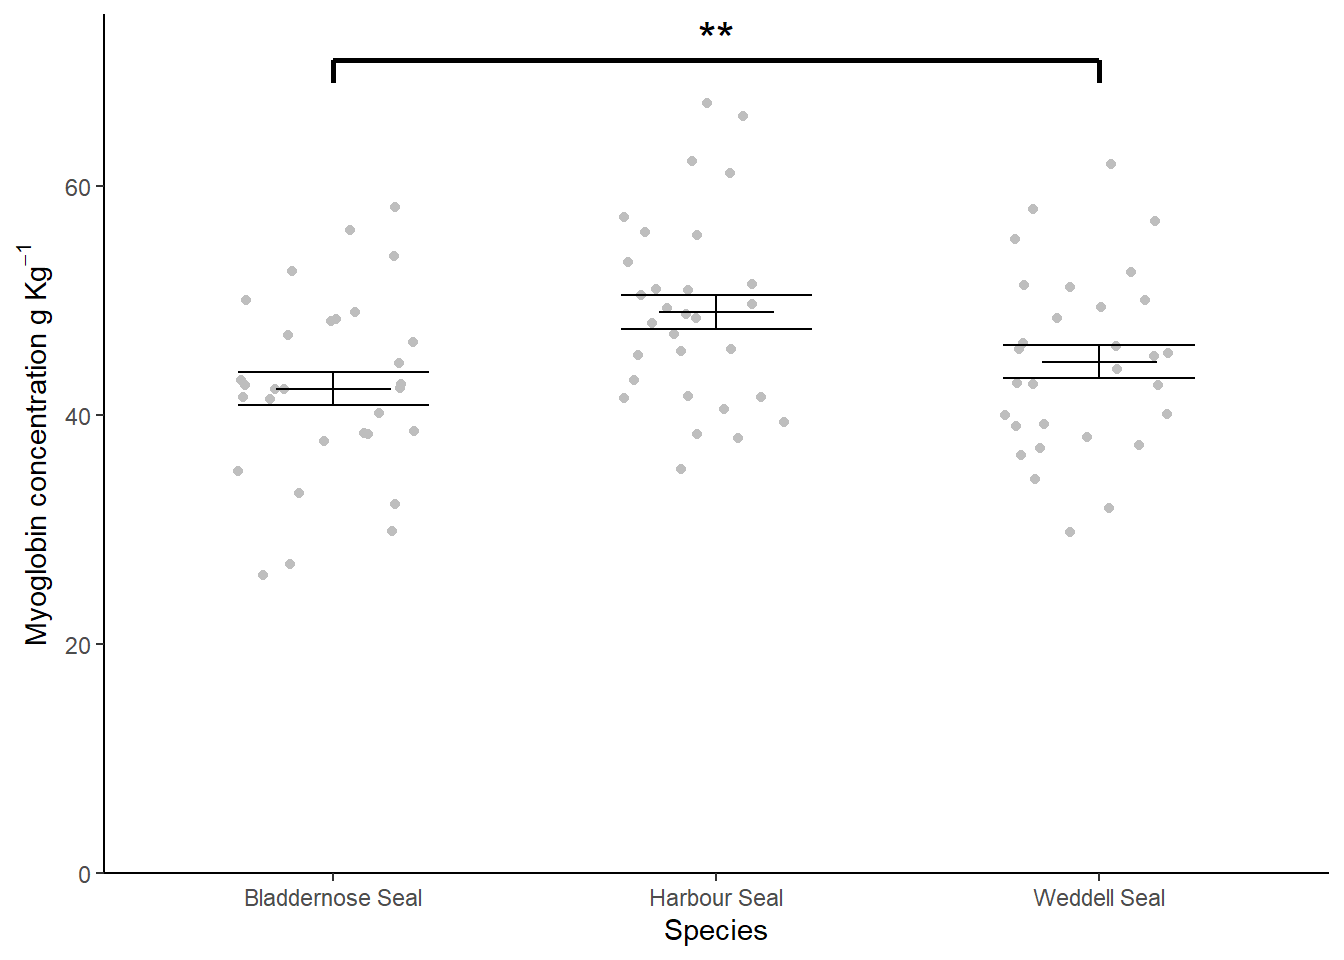
\includegraphics[width=0.8\linewidth]{one_way_anova_revisit_files/figure-latex/fig-one-anova-1} \end{flushleft}

\hypertarget{reporting-the-results-2}{%
\section{Reporting the results}\label{reporting-the-results-2}}

\begin{Shaded}
\begin{Highlighting}[]
\CommentTok{# res <- summary(mod)}
\CommentTok{# tval <- res$coefficients["specieswild", "t value"]}
\CommentTok{# df <- res$df[2]}
\end{Highlighting}
\end{Shaded}

There is a significant difference in myoglobin concentration between Seal species (ANOVA: \(F\) = 5.352; \(d.f.\) = 2, 87; \$p \(= 0.006). Post-hoc testing revealed that difference to be between the Harbour Seal with the highest myoglobin concentrations (\)\bar\{x\} \pm s.e.\$: 49.0103333333333 \(\pm\) 1.50660289891503) ) and the Bladdernose Seal with the lowest (\(\bar{x} \pm s.e.\): 42.316 \(\pm\) 1.46436064272228). See figure \ref{fig:fig-one-anova-report}.



\begin{figure}

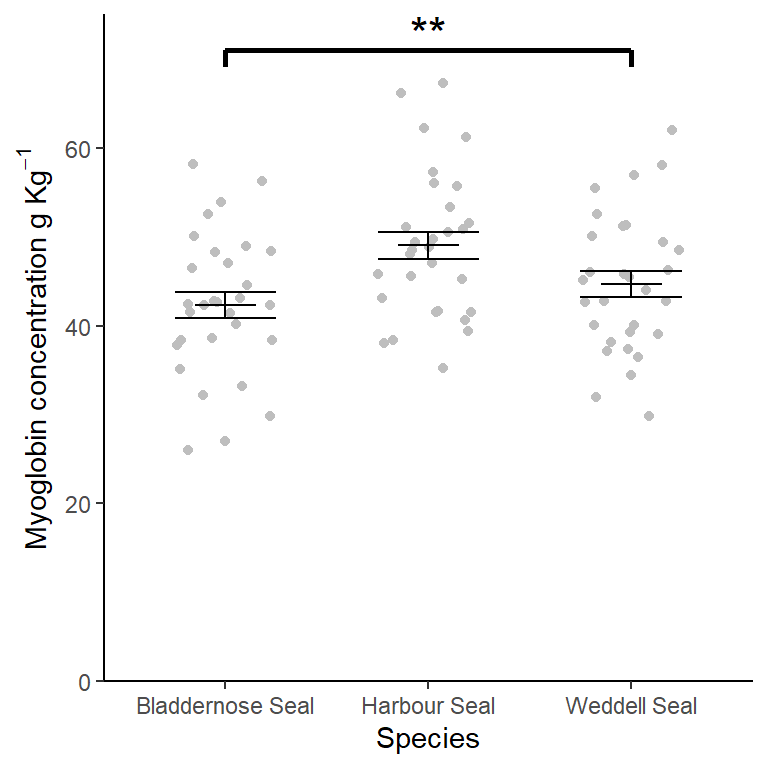
\includegraphics[width=0.8\linewidth]{one_way_anova_revisit_files/figure-latex/fig-one-anova-report-1} \hfill{}

\caption{Muscle myoglobin content of three seal species.}\label{fig:fig-one-anova-report}
\end{figure}

\hypertarget{two-way-anova-revisit}{%
\chapter{Two-way ANOVA revisited}\label{two-way-anova-revisit}}

\hypertarget{introduction-to-the-example-3}{%
\section{Introduction to the example}\label{introduction-to-the-example-3}}

\begin{Shaded}
\begin{Highlighting}[]
\KeywordTok{library}\NormalTok{(tidyverse)}
\end{Highlighting}
\end{Shaded}

\hypertarget{t.test-output-reminder-1}{%
\section{\texorpdfstring{\texttt{t.test()} output reminder}{t.test() output reminder}}\label{t.test-output-reminder-1}}

\hypertarget{applying-and-interpreting-lm-3}{%
\section{\texorpdfstring{Applying and interpreting \texttt{lm()}}{Applying and interpreting lm()}}\label{applying-and-interpreting-lm-3}}

\hypertarget{getting-predictions-from-the-model-3}{%
\section{Getting predictions from the model}\label{getting-predictions-from-the-model-3}}

\hypertarget{checking-assumptions-3}{%
\section{Checking assumptions}\label{checking-assumptions-3}}

\hypertarget{creating-a-figure-3}{%
\section{Creating a figure}\label{creating-a-figure-3}}

\hypertarget{reporting-the-results-3}{%
\section{Reporting the results}\label{reporting-the-results-3}}

\hypertarget{part-glm-for-poisson-responses}{%
\part{GLM for Poisson responses}\label{part-glm-for-poisson-responses}}

\hypertarget{pois}{%
\chapter{GLM for poisson responses}\label{pois}}

\hypertarget{pois-intro}{%
\section{intro}\label{pois-intro}}

some stuff introducing pois

\hypertarget{pois-build}{%
\section{build}\label{pois-build}}

some stuff about build pois

\hypertarget{pois-output}{%
\section{output}\label{pois-output}}

some stuff about pois output

\hypertarget{part-glm-for-binomial-responses}{%
\part{GLM for binomial responses}\label{part-glm-for-binomial-responses}}

\hypertarget{bino}{%
\chapter{GLM for binomial responses}\label{bino}}

\hypertarget{bino-intro}{%
\section{intro}\label{bino-intro}}

some stuff introducing bino

\hypertarget{bino-build}{%
\section{build}\label{bino-build}}

some stuff about build bino

\hypertarget{bino-output}{%
\section{output}\label{bino-output}}

some stuff about bino output

\hypertarget{summary}{%
\chapter{Summary}\label{summary}}

key points

where to go next

  \bibliography{refs/book.bib,refs/packages.bib}

\end{document}
